\documentclass[14pt, a4paper]{article}
\usepackage[T2A]{fontenc}
\usepackage[utf8]{inputenc}
\usepackage[russian]{babel}
\usepackage[left=3cm, right=1.5cm, top=2cm, bottom=2cm]{geometry}
\usepackage{indentfirst}
\usepackage{microtype}
\usepackage{array}
\usepackage{xcolor}
% \usepackage{times}
\usepackage{tempora}
\usepackage{ulem}
\usepackage{setspace}
\usepackage{amsmath}
\usepackage{booktabs}
\usepackage{graphicx}
\usepackage{float}
\usepackage{listings}
\graphicspath{{reports/figures/}{figures/}}
\lstset{basicstyle=\ttfamily\small, breaklines=true, columns=fullflexible, frame=single, keepspaces=true}
\pagestyle{empty}

\makeatletter
\renewcommand\section{\@startsection {section}{1}{\parindent}%
  {-3.5ex \@plus -1ex \@minus -.2ex}%
  {0.5ex}%
  {\normalfont\Large\bfseries}}
\renewcommand\tableofcontents{%
  \begin{center}\Large\bfseries\contentsname\end{center}%
  \@starttoc{toc}%
}
\renewcommand*\l@section{\@dottedtocline{1}{0em}{1.5em}}
\makeatother

\begin{document}
\onehalfspacing

\begin{center}
    \textbf{ФЕДЕРАЛЬНОЕ ГОСУДАРСТВЕННОЕ АВТОНОМНОЕ ОБРАЗОВАТЕЛЬНОЕ} \\
    \textbf{УЧРЕЖДЕНИЕ ВЫСШЕГО ОБРАЗОВАНИЯ} \\
    \textbf{«МОСКОВСКИЙ АВИАЦИОННЫЙ ИНСТИТУТ} \\
    \textbf{(НАЦИОНАЛЬНЫЙ ИССЛЕДОВАТЕЛЬСКИЙ УНИВЕРСИТЕТ)»}
\end{center}

\begin{center}
    \bfseries Институт №8 «Компьютерные науки и \\
    \bfseries прикладная математика» \\
    \bfseries Кафедра 806 «Вычислительная математика \\
    \bfseries и программирование»
\end{center}

\vspace{3cm}

\begin{center}
    \Large\bfseries Отчет \\
    \vspace{0.5cm}
    \mdseries по лабораторной работе №3.2
\end{center}

\vfill

\noindent
\hfill
\begin{tabular}{ll}
Группа:       & М8О-307Б-21 \\
Студент:      & М. С. Ивченко \\
Преподаватель:& доц. В. В. Киндинова \\
Оценка:       & \underline{\makebox[3cm][c]{}} \\ [0.2cm]
Дата:         & \underline{\makebox[3cm][c]{}}
\end{tabular}

\vfill

\begin{center}
    Москва \\
    2026
\end{center}

\newpage

\setcounter{tocdepth}{2}
\tableofcontents
\newpage

\section*{Тема}
\addcontentsline{toc}{section}{Тема}
Цель данной лабораторной работы -- познакомиться с гладкой кусочной интерполяцией табличных данных. Кубический сплайн позволяет получить плавную кривую между узлами, избегая чрезмерных колебаний, характерных для многочленов высокой степени.

\section*{Задание}
\addcontentsline{toc}{section}{Задание}
Построить кубический сплайн для функции, заданной в узлах интерполяции, предполагая, что сплайн имеет нулевую кривизну при $x = x_0$ и $x = x_4$. Вычислить значение функции в точке $x = X^*$.

\section*{Теория}
\addcontentsline{toc}{section}{Теория}
Полиномиальная интерполяция высокой степени может сильно колебаться между узлами. Кубический сплайн решает эту проблему иначе: вместо одного многочлена на всем отрезке строится набор кубических многочленов, по одному на каждый промежуток $[x_i,x_{i+1}]$:
\[
    S_i(x)=a_i+b_i(x-x_i)+c_i(x-x_i)^2+d_i(x-x_i)^3
\]
Коэффициенты подбираются так, чтобы сплайн проходил через все табличные точки и был гладким. В каждом внутреннем узле выполняются условия непрерывности функции, первой и второй производных:
\[
    S_{i-1}(x_i)=S_i(x_i),\quad
    S_{i-1}'(x_i)=S_i'(x_i),\quad
    S_{i-1}''(x_i)=S_i''(x_i).
\]

Для натурального сплайна дополнительно задается нулевая кривизна на концах:
\[
    S''(x_0)=0,\qquad S''(x_n)=0.
\]
Это означает, что на границах график не имеет искусственного изгиба. Если обозначить $h_i=x_i-x_{i-1}$, то неизвестные коэффициенты $c_i$, связанные со вторыми производными, находятся из трехдиагональной системы
\[
    h_i c_{i-1}+2(h_i+h_{i+1})c_i+h_{i+1}c_{i+1}
    =3\left(\frac{y_{i+1}-y_i}{h_{i+1}}-\frac{y_i-y_{i-1}}{h_i}\right).
\]
После нахождения $c_i$ остальные коэффициенты выражаются явно через соседние значения функции. Благодаря трехдиагональной структуре систему удобно решать методом прогонки.

\begin{lstlisting}[language=Python]
c[1:-1] = thomas_algorithm(system, right_side)
a = y[:-1].copy()
b = np.diff(y) / h - h * (c[1:] + 2 * c[:-1]) / 3
d = np.diff(c) / (3 * h)
\end{lstlisting}

\section*{Ход лабораторной работы}
\addcontentsline{toc}{section}{Ход лабораторной работы}
Для варианта заданы узлы
\[
\begin{array}{c|ccccc}
i&0&1&2&3&4\\\hline
x_i&-3&-1&1&3&5\\
y_i&2.8198&2.3562&0.78540&0.32175&0.19740
\end{array}
\]
и точка $X^*=-0.5$.

\begin{table}[H]
\centering
\begin{tabular}{c|rrrr}
\toprule
Отрезок & $a_i$ & $b_i$ & $c_i$ & $d_i$\\
\midrule
$[-3,-1]$&2.819800&-0.047003&0.000000&-0.046199\\
$[-1,1]$&2.356200&-0.601395&-0.277196&0.092597\\
$[1,3]$&0.785400&-0.599019&0.278384&-0.047394\\
$[3,5]$&0.321750&-0.054205&-0.005977&0.000996\\
\bottomrule
\end{tabular}
\caption{Коэффициенты натурального кубического сплайна.}
\end{table}
Вычисленное значение в заданной точке: $S(-0.5)=1.9977782645$.

\begin{figure}[H]
    \centering
    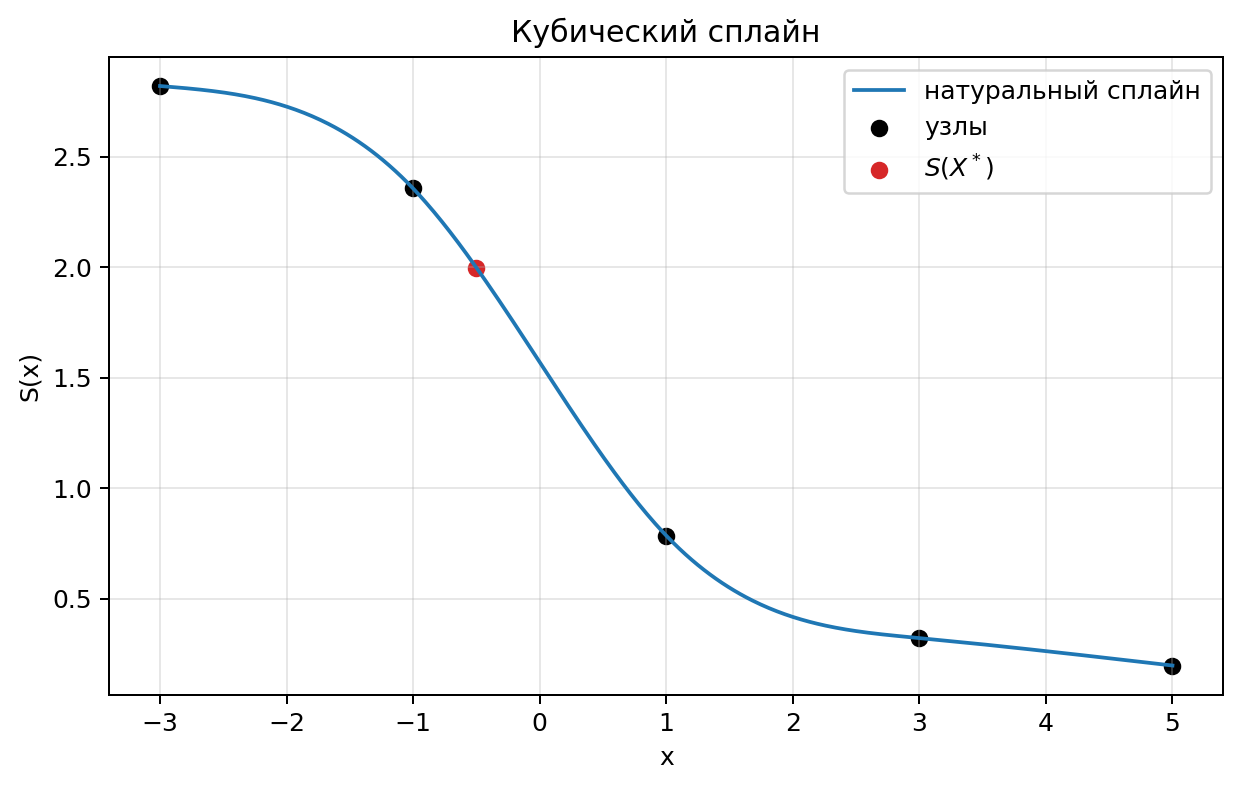
\includegraphics[width=0.86\textwidth]{lab3_2_spline.png}
    \caption{Натуральный кубический сплайн и значение в точке $X^*$.}
\end{figure}

\section*{Выводы}
\addcontentsline{toc}{section}{Выводы}
Натуральный кубический сплайн плавно проходит через все табличные точки и дает значение $1.9977782645$ в точке $-0.5$. Использование метода прогонки для коэффициентов удобно, поскольку система для сплайна трехдиагональная.

\end{document}
